\section{设计和测试过程中的场景术语}
\label{terminologie}
%
%As stated in the previous section, the requirements on the type of scenario representations in the development process of the ISO~26262 standard are contradictory.
正如上一节所述,在ISO 26262标准的开发过程中应用场景时,对场景的细节程度的需求是存在矛盾的。
%In the following section, the authors will suggest three abstraction levels for scenarios and show how these abstraction levels can be converted into each other along the development process.
在下一节中,作者将为场景建议三个抽象级别,并展示如何在开发过程中将这些抽象级别相互转换。
%Fig. \ref{fig:Abstraktionsebenen} illustrates the three levels of abstraction for scenarios: \textit{functional scenarios}, \textit{logical scenarios}, and \textit{concrete scenarios}.
作者将场景划分为三个抽象级别:功能场景(Functional scenarios)、逻辑场景(Logical scenarios)和具体场景(Concrete scenarios),如图\ref{fig:Abstraktionsebenen}所示。

\begin{figure*}
	\centering
	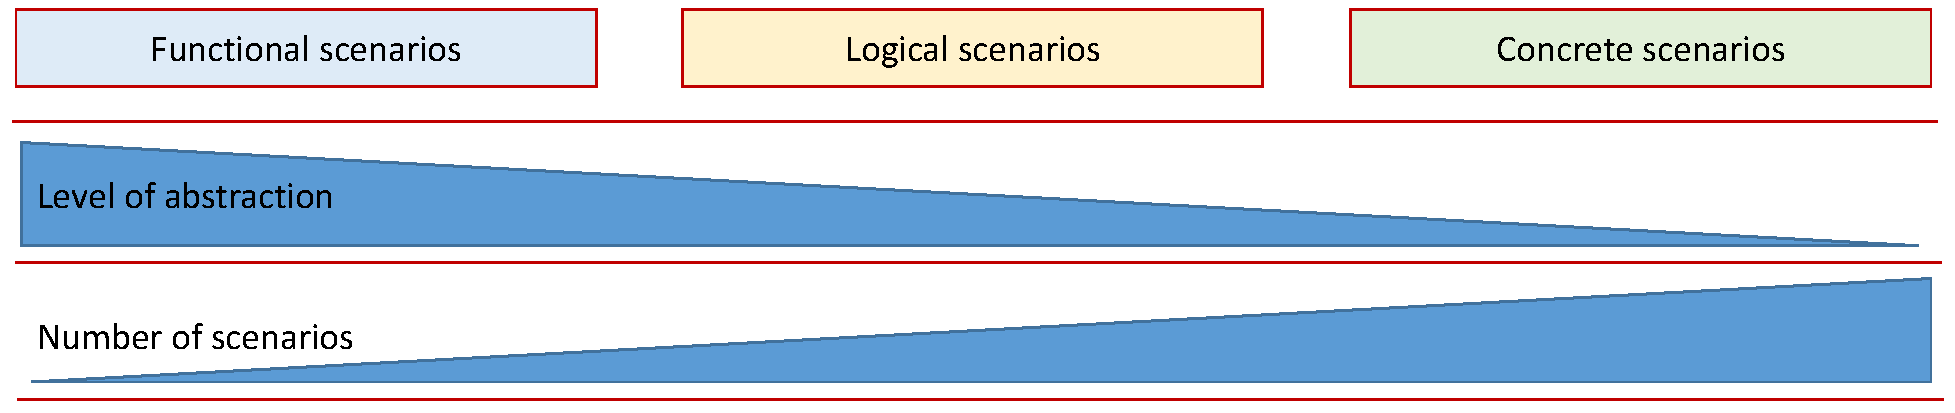
\includegraphics[width=1.0\textwidth]{./4_terminology/graphics/Abstraktionsebenen_reduziert2}
	\caption{ISO~26262标准开发过程中的抽象程度}
	\label{fig:Abstraktionsebenen}
\end{figure*}

\subsection{功能场景}
%Functional scenarios depict the most abstract level of scenario representations.
功能场景是场景表述的最抽象级别。
%These scenarios may be used for the item definition and the hazard analysis and risk assessment during the concept phase of the ISO~26262 standard.
在概念阶段,这些场景可用于项目定义、危险分析和风险评估。
%They are represented by language to ensure that human experts can easily understand existing scenarios, discuss them, and create new scenarios. 
它们以语言表示,以确保人类专家可以轻松理解现有场景,讨论它们并创建新场景。
%The authors suggest the following definition:
作者提出了以下定义:
\begin{quote}
\textit{
%Functional scenarios include operating scenarios on a semantic level.
功能场景包括语义级别的操作场景。
%The entities of the domain and the relations of those entities are described via a linguistic scenario notation.
通过语言场景符号来描述域内的实体以及实体间的关系。
%The scenarios are consistent.
场景是一致的。
%The vocabulary used for the description of functional scenarios is specific for the use case and the domain and can feature different levels of detail.
用于描述功能场景的术语表应由一般用例或域内专用的术语组成,并且可以具有不同的详细程度。
}
\end{quote}

%The representation of functional scenarios on a semantic level includes a linguistic and consistent description of entities and relations/interactions of those entities.
%For the linguistic description a consistent vocabulary has to be defined.
%This vocabulary includes terms for different entities (vehicle A, vehicle B) and phrases for the relations of those entities (vehicle A overtakes vehicle B). 
功能场景的表述包括实体和实体之间的关系,不同场景的描述方式必须是一致的。首先需要制定一个术语表,这个术语表包括不同实体的术语(车辆A、车辆B)和这些实体的关系短语(车辆A超越车辆B)。 

%The required level of detail of functional scenarios depends on the actual development phase and the item under development.
%Both aspects must be considered during the definition of the vocabulary.
功能方案所需的详细程度取决于实际开发阶段和正在开发的项目。在词术语表的定义过程中必须考虑这两个方面。
%For example, a highway pilot requires a vocabulary to describe the road geometry and topology, interactions with other traffic participants, and weather conditions. 
例如,高速公路飞行员需要术语表来描述道路几何形状和拓扑结构,与其他交通参与者的交互以及天气状况。
%On the contrary, a parking garage pilot requires a vocabulary to describe the layout of the building whereas weather conditions may be irrelevant.
相反,停车库行驶需要术语表来描述建筑物的布局,而天气条件可能是无关紧要的。
%If a comprehensive vocabulary is used for the description of the entities and the relations of those entities, a large amount of scenarios can be derived from the vocabulary.
如果使用综合术语表来描述实体和这些实体的关系,则可以从术语表中导出大量场景。
%For a generation of consistent functional scenarios, all terms of the vocabulary have to be distinct.
对于一致的功能场景泛化,术语表的所有术语必须是不同的。
%Sources for terms that define the entities of a domain are, for example, actual standards and guidelines like road traffic regulations or the German standard for constructing motorways
定义域实体的术语来源是,例如,道路交通法规或德国高速公路建设标准等实际标准和指南\cite{RAA}。

\begin{figure}
	\centering
	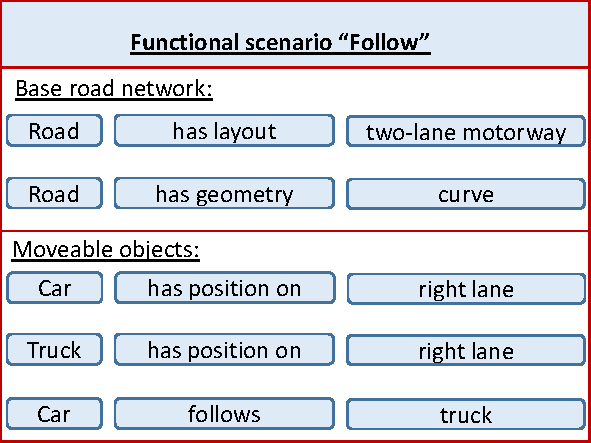
\includegraphics[width=0.9\columnwidth]{./4_terminology/graphics/functionalScenario.pdf}
	\caption{在高速公路行驶的一个功能场景:一辆轿车和一辆卡车正行驶在右侧车道上,轿车跟随卡车行驶。}
	\label{fig:functionalScenario}
\end{figure}

%Fig. \ref{fig:functionalScenario} shows a functional scenario for a highway pilot on a two-lane motorway in a curve.
%A car and a truck are driving on the right lane of the road, whereby the car follows the truck.
%In this example, the road is described with a layout and a geometry.
图\ref{fig:functionalScenario}为在高速公路行驶的一个功能场景:一辆轿车和一辆卡车正行驶在右侧车道上,轿车跟随卡车行驶。在这个例子中,道路特征主要描述为横断面布置情况和几何结构特征。
%Depending on the item's use case and domain, the vocabulary has to include additional terms to describe these characteristics like `three-lane motorway' for layout, and `straight' or `clothoid' for geometry.
根据项目的用例和域,词汇表必须包含用于描述这些特征的附加术语,例如用于布局的“三车道高速公路”,以及用于几何的“直线”或“回旋曲线”。
%The scenario can be varied by choosing other terms from the defined vocabulary.
通过从定义的术语表中选择其他术语,可以改变场景。
\subsection{逻辑场景}
%Logical scenarios depict a detailed representation of functional scenarios with the help of state space variables.
基于状态空间变量,逻辑场景是对功能场景的进一步详细描述。
%Hence, functional scenarios can be converted into a representation which is based on parameters. 
%Those state space variables describe the entities and the relations of those entities.
那些状态空间变量描述了这些实体的实体和关系。
%Logical scenarios may be used to derive and represent requirements for the item during the system development phase.
在系统开发阶段,可以利用逻辑场景派生出安全需求。
%For that purpose, logical scenarios describe the value ranges of the state space variables via a formal notation.
为此,逻辑场景通过正式表示法描述状态空间变量的值范围。
%The authors suggest the following definition for logical scenarios:
作者提出了以下定义:
\begin{quote}
\textit{
%Logical scenarios include operating scenarios on a state space level.
%Logical scenarios represent the entities and the relations of those entities with the help of parameter ranges in the state space.
%The parameter ranges can optionally be specified with probability distributions.
%Additionally, the relations of the parameter ranges can optionally be specified with the help of correlations or numeric conditions.
%A logical scenario includes a formal notation of the scenario.
逻辑场景以状态空间呈现操作场景。通过定义状态空间内变量的参数范围,可以表达实体特征和实体间的关系。参数范围可以选择用概率分布来确定。此外,不同参数的关系可以通过相关性或数值条件来确定。逻辑场景应包含该场景的形式标记。
}
\end{quote}

%The logical scenario description covers all elements necessary for the derivation of technical requirements needed to implement a system which solves these scenarios.
逻辑场景涵盖了提出安全需求所需的所有元素。
%For a step-wise specification of scenarios in the development process of the ISO~26262 standard, logical scenarios have to be described via a formal notation in the state space, whereby parameters have to be defined via value ranges.
为了在标准规定的开发过程中逐步规范场景,必须在状态空间中通过形式标记来表述逻辑场景,并从取值范围中确定参数。
%the linguistic representation of functional scenarios has to be converted to the formal state space notation of logical scenarios.  
%The state space of logical scenarios is described via parameters and value ranges for those parameters.
%For a more detailed description of those parameter ranges, probability distributions (e.g., Gaussian distribution, Uniform distribution) can optionally be specified for each parameter range.
可以通过概率分布(例如,高斯分布,均匀分布)为每个参数指定范围。
%Additionally, relations of the parameter ranges can optionally be specified by numeric conditions (e.g., the speed of an overtaking vehicle has to be greater than the speed of the overtaken vehicle) or correlation functions (e.g., lane width correlates with curve radius).
参数范围间的关系可以由数值条件或相关函数来指定(例如,超车速度必须大于被超车速度,车道宽度与曲线半径相关)。

\begin{figure}
	\centering
	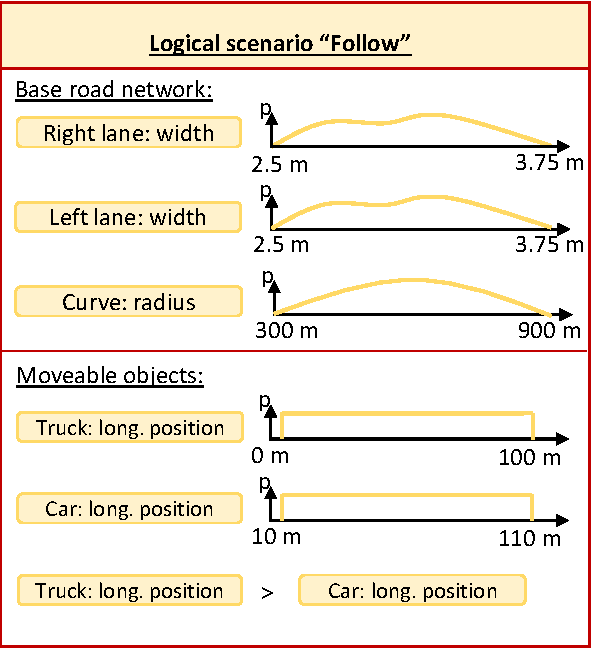
\includegraphics[width=0.9\columnwidth]{./4_terminology/graphics/logicalScenario.pdf}
	\caption{逻辑场景的示例。 一辆汽车沿着双车道高速公路右侧车道的一辆卡车行驶。}
	\label{fig:logicalScenario}
\end{figure}

%Fig. \ref{fig:logicalScenario} shows a logical scenario that has been derived from the functional scenario illustrated in Fig. \ref{fig:functionalScenario}.
图\ref{fig:logicalScenario}显示了从图\ref{fig:functionalScenario}所示的功能场景中衍生出的逻辑场景。
%Functional scenarios are converted to logical scenarios by a transformation from the linguistic representation into state space and specification of the scenario describing parameters.
通过从语言表述到状态空间的转换以及描述参数的场景的规范,功能场景被转换为逻辑场景。
%Hence, every term from the vocabulary has to be assigned to parameters which describe this term.
因此,功能场景术语表中的每一项都必须分配一个描述该术语的参数。
%In this example, both lanes are described via a lane width, the curve geometry is represented by a radius, and the vehicles are described by longitudinal positions along the lane.
%Furthermore, the term `follows' demands that the longitudinal position of the truck is greater than the longitudinal position of the car.
在这个例子中,两条车道都是通过车道宽度来描述的,几何结构是由一个半径来表示的,车辆由其纵向位置来描述,并要求卡车纵向位置大于轿车。本文作者选择了一组简化的参数。在实际应用中,可能需要多个参数来描述单个术语,例如,一辆卡车可以通过规定其尺寸、重量和发动机功率来定义。
%To allow the example to be reflected in this paper, the authors have chosen a reduced set of parameters.
%
%%Hence, the example can be handled in this paper, the authors have chosen a very narrow parameter space.
%In reality, much more parameters will be necessary to describe a single term from the vocabulary.
%%In reality there will be much more parameters necessary to describe a single term from the vocabulary.
%For example, a truck can additionally be specified by its dimensions, weight, and engine power.

%In addition, for every parameter from the example in Fig.~\ref{fig:logicalScenario} the value range and the probability distribution, with which the parameter occurs in reality, are specified.
另外,对于图~\ref {fig:logicalScenario}中的示例的每个参数,指定了值范围和参数实际出现的概率分布。
%This information helps to formulate technical requirements in the system development phase and provide a basis for a systematic generation of concrete scenarios in the testing phase.
该信息有助于在系统开发阶段制定技术要求,并为在测试阶段系统生成具体方案提供基础。

%
%\todo{Logical scenarios are scenarios, which describe an episode of traffic on a semi-formal level. The scenario description covers all elements necessary for the derivation of technical requirements to implement a system, which solves these scenarios. Logical scenarios include parameter descriptions and ranges for all elements of the scenario, including related probability distributions of parameter values.}
%\todo{AR: Enthalten logische Szenarien auch Informationen über die Beziehungen zwischen Elementen des Szenarios oder nicht? Z.B.: Tempolimit für Fahrstreifen versus Fahrstreifen und Schild ohne Beziehung zueinander?}
%\todo{AR: Folgenden Satz würde ich nach der Definition anhängen, da er ja nicht teil der Definition ist: The parameter space and the value ranges can be derived from the abstract linguistic representaion of functional scenarios and have to be defined distinctly.}

\subsection{具体场景}
%Concrete scenarios describe the entities and the relations for those entities using distinct parameters in the state space.
具体场景由某个确定的参数值来表示状态空间中实体和实体间关系
%Every logical scenario can be converted to a concrete scenario by selection of a concrete value from a parameter range.
每个逻辑场景都可以通过从参数范围中选择具体值来转换为具体场景。
%Concrete scenarios may be used as a basis for test case generation in the testing phase.
具体场景可以作为测试用例的基础。作者提出了以下定义:
%The authors suggest the following definition for concrete scenarios:

\begin{quote}
\textit{
%Concrete scenarios distinctly depict operating scenarios on a state space level.
%Concrete scenarios represent entities and the relations of those entities with the help of concrete values for each parameter in the state space.
具体场景以状态空间详细描述了操作场景。通过确定状态空间中每个参数的具体值来明确描述实体和实体间的关系。
}
\end{quote}

%For each logical scenario with continuous value ranges any number of concrete scenarios can be derived.
对于每一个具有连续取值范围的逻辑场景,都可以派生出任意数量的具体场景。
%For example, an infinite number of concrete scenarios can be achieved by choosing an infinitesimal sampling step width for each parameter.
例如,通过为每个参数选择无穷小的采样步长,可以实现无限数量的具体场景。
%An efficient concretization is accomplished by identification and combination of representative discrete values for each parameter.
为保证生成具体场景的效率,应选择有代表性的离散值进行组合。
%Only concrete scenarios can directly be converted into test cases and executed with a vehicle guidance system.
必须强调的是,只有具体场景可以直接转化为测试用例。

\begin{figure}
	\centering
	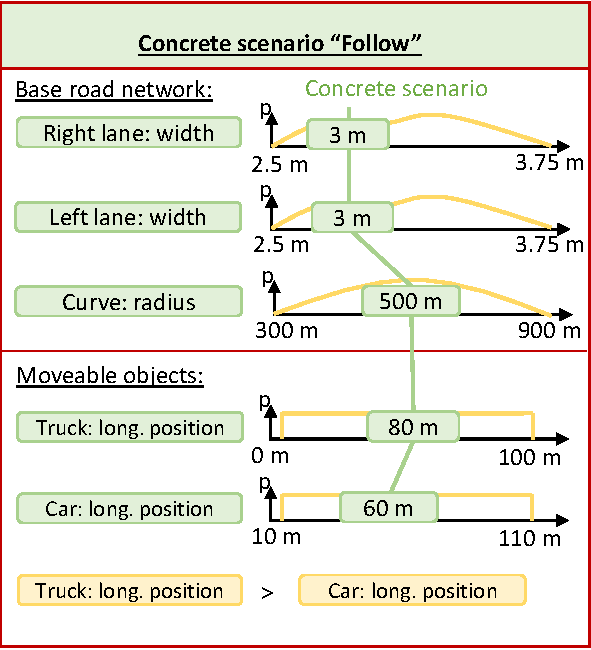
\includegraphics[width=0.9\columnwidth]{./4_terminology/graphics/concreteScenario.pdf}
	\caption{具体场景示例。一辆汽车沿着双车道高速公路右侧车道的一辆卡车行驶。}
	\label{fig:concreteScenario}
\end{figure}

%Fig. \ref{fig:concreteScenario} shows a concrete scenario that has been derived from the logical scenario illustrated in Fig. \ref{fig:logicalScenario}.
图\ref{fig:concreteScenario}为一个具体的场景,该场景由图\ref{fig:logicalScenario}中所示的逻辑场景衍生。
%For every parameter, a concrete value within the value range has been chosen.
%Logical scenarios are converted to concrete scenarios by choosing a concrete value within the value range for each parameter.
%For every parameter a concrete value within the defined value range has been chosen while the specified condition regarding the parameters has been satisfied.
对于每个参数,已经选择了在定义的值范围内的具体值,同时满足了关于参数的指定条件。
%To transform concrete scenarios into test cases, concrete scenarios have to be augmented by the expected behavior of the test object and the test infrastructure to be used as stated by Ulbrich~et~al.~\cite{ulbrich_definition_2015}.
%The expected behavior can be derived from the functional operating scenarios, the logical scenarios, or the item definition. 
要将具体场景转换成测试用例,需要增加被测对象的预期行为表现,以及对相关测试设施的需求~\cite{ulbrich_definition_2015}。而被测对象的预期行为则可以从操作场景、逻辑场景或项目定义中导出。
%
%\subsection{Integration of the scenario definitions into the development process}
%
%\begin{figure*}[b!]
%	\centering
%	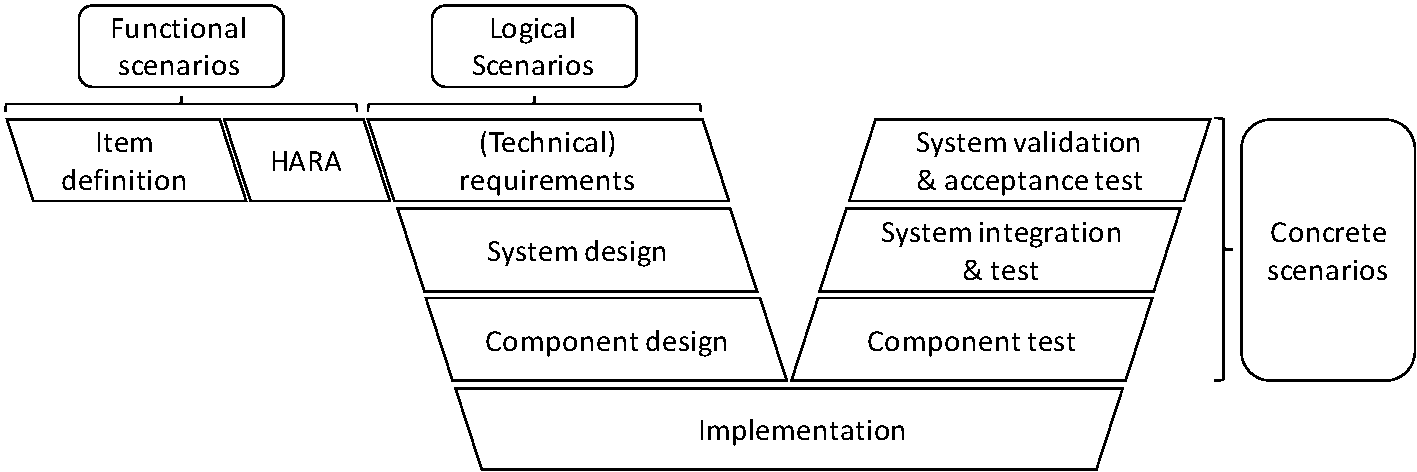
\includegraphics[width=0.75\textwidth]{./4_terminology/graphics/V_Modell}
%	\caption{Functional, logical and concrete scenarios in the V-model-based development process; HARA: Hazard analysis and risk assessment}
%	\label{fig:Prozess}
%\end{figure*}

%
%In the concept phase, functional scenarios are used to define the operating scenarios of the item and build a basis for a hazard analysis and risk assessment.
%To enable human experts to discuss about occurring risks, functional scenarios are represented in a linguistic way.

%Functional, logical, and concrete scenarios can be converted into each other.
%Functional scenarios can be converted to logical scenarios by a transformation from the linguistic representation into state space and specification of the scenario describing parameters.
%Logical scenarios can be converted to concrete scenarios by concretization of each parameter range to a concrete value.
%Fig. \ref{fig:Prozess} shows a schematic development process based on the V-model with the suggested levels of scenario abstraction.
%
%Before the technical development starts, functional scenarios are used for the item definition and the hazard analysis and risk assessment.
%Functional scenarios are represented linguistically and have to be converted to logical scenarios by a transformation into the state space and specification of the scenario describing parameters.
%Within this context, technical requirements can be formulated by valid and invalid value ranges of the parameters describing the scenario respectively.
%
%
%Concrete scenarios are the basis for executable test cases.
%A test case contains a concrete scenario and additionally the pass/fail criteria, which result from the desired behavior of the system under test. In logical scenarios, the possible parameters of all movable objects are available in the parameter ranges. Thus, the desired behavior of the ego vehicle can't be derived in general, since it is different for specific parameter sets.
%To transform concrete scenarios into test cases, concrete scenarios have to be augmented by the expected behavior of the test object and the test infrastructure to be used as stated by Ulbrich~et~al.~\cite{ulbrich_definition_2015}.
%The expected behavior can be derived from the functional operating scenarios, the logical scenarios, or the item definition. 
%
%A big difference of concrete scenarios and test cases is the representation of the behavior of the test object.
%Within a test case, the resulting behavior of the test object is not known. The resulting behavior first occurs, when the test case is executed.
%In concrete scenarios the behavior of all traffic participants is at least known by their goals and values.




